\section{Introduction}
\label{sec:introduction}

% state the learning objective 
The objective of this laboratory assignment is to study a circuit containing two independent and two linearly dependent sources. $V_a$ is the independent voltage source and $I_d$ is the independent current source.
\par The voltage controlled current source $I_b$ is determined by $K_b \cdot V_b$, and the current controlled voltage source $V_c$ is calculated with $K_c \cdot I_c$.
The circuit can be seen in Figure \ref{fig:Circuit}, where it is found that along with these sources, the circuit is composed of seven more resistors, named $R_1$, $R_2$, ..., $R_7$.
\par The resistor values were obtained from a \textit{Python} script, given by the professor and using the student number 95802 to generate the data. These values are shown in the table below, where names starting with R represent resistors, and the units are \textit{kOhm} (kiloohm). $K_b$ is given in \textit{mS} (millisiemens), whereas $K_c$ is expressed in \textit{kOhm}. $V_a$ and $I_c$ are expressed in \textit{V} (volt) and \textit{mA} (milliampere), respectively.
 
\par

\begin{center}
\begin{tabular}{ |c|c|c| }
 \hline
\textbf{Name} & \textbf{Value} \\
 \hline
 $R_{1}$ & 1.01658203395 \\
 \hline
 $R_{2}$ &  2.08071598482 \\
 \hline
 $R_{3}$ & 3.12527703197  \\
 \hline
 $R_{4}$ & 4.13615246449\\
 \hline
 $R_{5}$ & 3.04804224053  \\
 \hline
 $R_{6}$ & 2.06609096892 \\
 \hline
 $R_{7}$ & 1.01589064139\\
 \hline
 $K_{b}$ & 7.30340439475\\
 \hline
 $K_{c}$ & 8.13276803722\\
 \hline
 $V_{a}$ & 5.08211987776 \\
 \hline
 $I_{c}$ & 1.02439571082 \\
 \hline
\end{tabular}
\end{center}


In Section~\ref{sec:analysis}, two theoretical analysis of the circuit are
presented, using the mesh method and the node method. In Section~\ref{sec:simulation}, the circuit is analysed by
simulation, and the results are compared to the theoretical results obtained in
Section~\ref{sec:analysis}. The conclusions of this study are outlined in
Section~\ref{sec:conclusion}.

\begin{figure}[h] \centering
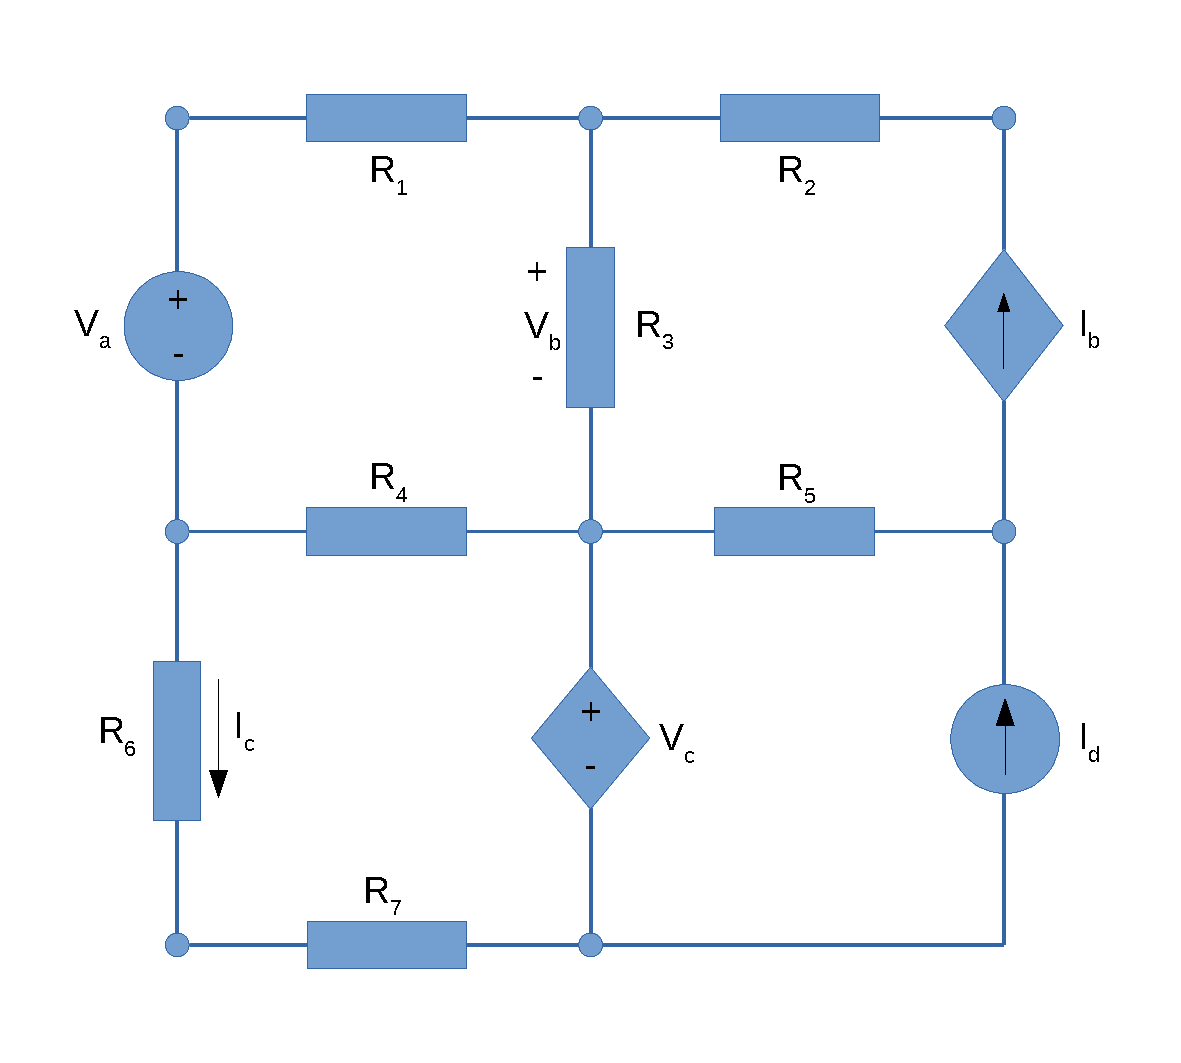
\includegraphics[width=0.5\linewidth]{Circuit.pdf}
\caption{T1 circuit.}
\label{fig:Circuit}
\end{figure}
